% -*- mode:flyspell; mode:latex -*-
\documentclass[12pt]{article}
\addtolength{\oddsidemargin} {-0.885in}
\addtolength{\textwidth}{1.75in}
\addtolength{\evensidemargin}{-0.8in}


\usepackage[latin1]{inputenc}
\usepackage[T1]{fontenc}
\usepackage[english]{babel}
\usepackage{graphicx}
\usepackage{float}
%% \usepackage{siunitx}

%% \usepackage{gensymb}


\usepackage{tikz}
\usepackage{[caption}
\usetikzlibrary{arrows}
\usetikzlibrary{decorations.markings}
\usetikzlibrary{decorations.pathmorphing}
% \usepackage[absolute,overlay]{textpos}
% \usepackage{onimage}

\usepackage{tabularx}
\usepackage{times}
\usepackage{graphics}

% \usepackage{subfigure}
% \usepackage{scalefnt}
%
% \renewcommand\thesubfigure{\arabic{subfigure}}

\usepackage{amsmath}
\usepackage{hyperref}
\usepackage{hhline}
\usepackage{subfig}
\usepackage{color}
\usepackage[all]{hypcap}

\usepackage[normalem]{ulem}  % for striking out
% \usepackage{fancyhdr}
% \pagestyle{fancy}
% \fancyhead[C]{}
% \fancyhead[L] {\it{Mu2e-doc-29670-v1.0} }
%%%%%%%%%%%%%%%%%%%%%%%%%%%%%%%%%%%%%%%%%%%%%%%%%%%%%%%%%%%%%%%%%%%%%%%%%%%%%%
% use natbib - biblatex not available on Mu2e interactive nodes
%%%%%%%%%%%%%%%%%%%%%%%%%%%%%%%%%%%%%%%%%%%%%%%%%%%%%%%%%%%%%%%%%%%%%%%%%%%%%%
\usepackage[square,sort,comma,numbers]{natbib}

% location of the .bib files: env var BIBINPUTS (~/library/bibliography)

% \usepackage[backend=biber, style=numeric-comp, sorting=ynt] {biblatex}
% \addbibresource{clfv.bib}

% \addbibresource{stntuple.bib}
% \addbibresource{mu2e_web.bib}
% \addbibresource{radiative_pion_capture.bib}

\graphicspath{{figures/}}
%%%%%%%%%%%%%%%%%%%%%%%%%%%%%%%%%%%%%%%%%%%%%%%%%%%%%%%%%%%%%%%%%%%%%%%%%%%%%%
% for portability, make sure all commands are included locally,
%%%%%%%%%%%%%%%%%%%%%%%%%%%%%%%%%%%%%%%%%%%%%%%%%%%%%%%%%%%%%%%%%%%%%%%%%%%%%%
\definecolor{ForestGreen}{RGB}{20,109,20}
%\include{commands}
\newcommand {\blue}      {\color{blue}}
\newcommand {\green}     {\color{ForestGreen}}
\newcommand {\red}       {\color{red}}
\newcommand {\purple}    {\color{purple}}
\newcommand {\violet}    {\color{violet}}

\newcommand {\kmax}      {\mbox{$k_{\rm max}$}}
\newcommand {\piplusenu} {\mbox{$\pi^+ \to e^+ \nu$}}

\newcommand {\mumemconv}[1][A] {\mbox{$\mu^- \textrm{#1} \rightarrow e^- \textrm{#1}$}}
% Define a relay to have 2 default arguments instead of limit of 1
\newcommand {\mumepconv}[1][A] {%
  \def\ArgI{{#1}}%store the first argument
  \mumepconvRelay
}
\newcommand \mumepconvRelay[1][A]  {\mbox{$\mu^- \textrm{\ArgI} \rightarrow e^+ \textrm{#1}$}}
\newcommand {\MuToEm}     {\mbox{$\mu^- \ra e^-$}}
\newcommand {\MuToEp}     {\mbox{$\mu^- \ra e^+$}}
\newcommand {\MuPToEp}    {\mbox{$\mu^+ \ra e^+$}}
\newcommand {\ra}        {\rightarrow}
\newcommand {\Rmue}       {\mbox{$R_{\mu e}$}}
\newcommand {\tandip}    {\mbox{$\tan \lambda$}}

\newcommand {\Pb}[1]     {\mbox{$\rm ^{#1}Pb$}}                 % isotopes of lead
\newcommand {\Au}[1]     {\mbox{$\rm ^{#1}Au$}}                 % isotopes of gold
\newcommand {\Ir}[1]     {\mbox{$\rm ^{#1}Ir$}}                 % isotopes of iridium
%%%%%%%%%%%%%%%%%%%%%%%%%%%%%%%%%%%%%%%%%%%%%%%%%%%%%%%%%%%%%%%%%%%%%%%%%%%%%%
% editing commands
%%%%%%%%%%%%%%%%%%%%%%%%%%%%%%%%%%%%%%%%%%%%%%%%%%%%%%%%%%%%%%%%%%%%%%%%%%%%%%
\newcommand {\del}[1]    {{\blue   \sout{#1}}}
\newcommand {\dlt}[1]    {{\violet \sout{#1}}} %alternate delete color
\newcommand {\add}[1]    {{\red #1}}
\newcommand {\alt}[1]    {{\green #1}} %alternate comment color
% %%%%%%%%%%%%%%%%%%%%%%%%%%%%%%%%%%%%%%%%%%%%%%%%%%%%%%%%%%%%%%%%%%%%%%%%%%%%%%
% for editors
% %%%%%%%%%%%%%%%%%%%%%%%%%%%%%%%%%%%%%%%%%%%%%%%%%%%%%%%%%%%%%%%%%%%%%%%%%%%%%%
\newcommand {\pasha}[1]    {{\green  #1}}
\newcommand {\kate}[1]     {{\blue   #1}}
%%%%%%%%%%%%%%%%%%%%%%%%%%%%%%%%%%%%%%%%%%%%%%%%%%%%%%%%%%%%%%%%%%%%%%%%%%%%%%
\begin{document}

\begin{titlepage}
  \begin{flushright}
    \bf {MU2E/PHYSICS/50203} \\
    version 1.01
    \today
 \end{flushright}

  \vspace{1cm}

  \begin{center}
    {\Large \bf On a role of TSdA4
      % \vspace{0.3in}
      % 1. Proof of principle
    }

    \vspace{1cm}
    P.Murat(FNAL)

    % \footnote{\texttt{Fermilab; e-mail: murat@fnal.gov}}
    \vspace{0.3cm}

    \vspace{0.8cm}
  \end{center}

  \begin{abstract}
    \vspace{0.2in}
    The TSdA is a 2-inch thick polyethylene disk introduced to shield the tracker
    from the neutron background. The motivation to introduce the TSdA was based
    on the MC simulation showing that TSdA reduces the number of hits in
    the tracker by 30\% \cite{MU2E_3479_NEUTRON_SHIELDING}.
%
    To better understand the mechanism of shielding, we attempted to reproduce
    this result.

    According to results of this study, the impact of the TSdA on the detector occupancy
    is very minimal.
    Adding TSdA reduces the neutron-induced number of hits in the tracker by about 4\%,
    and the total number of hits in the tracker by less than 2\%.
    For the calorimeter, the corresponding numbers are below 1\%
%
    This simulation shows that the TSdA doesn't absorb the neutrons emitted
    in the muon captures. Instead, it blocks low-energy electrons produced
    in the TS, preventing electrons from entering  the tracker.

  \end{abstract}

\end{titlepage}
% \frontmatter
% \chapter*{Abstract}
%
% \addcontentsline{toc}{chapter}{Abstract}
%
% \mainmatter
%
{\tableofcontents}

%%%%%%%%%%%%%%%%%%%%%%%%%%%%%%%%%%%%%%%%%%%%%%%%%%%%%%%%%%%%%%%%%%%%%%%%%%%%%%%
%\chapter{Calibration}
%%%%%%%%%%%%%%%%%%%%%%%%%%%%%%%%%%%%%%%%%%%%%%%%%%%%%%%%%%%%%%%%%%%%%%%%%%%%%%%
% \input{input_data}

%%%%%%%%%%%%%%%%%%%%%%%%%%%%%%%%%%%%%%%%%%%%%%%%%%%%%%%%%%%%%%%%%%%%%%%%%%%%%%%
% 
% \newpage
% \section {Revision History and TODO items}
% 
% \begin{itemize}
% \item
%   v1.01: inital version
% \end{itemize}
% 
%%%%%%%%%%%%%%%%%%%%%%%%%%%%%%%%%%%%%%%%%%%%%%%%%%%%%%%%%%%%%%%%%%%%%%%%%%%%%%
\newpage
\section {Introduction}

TSdA (TSd Absorber) is a 2-inch th.ick polyethylene disk positioned right
on exit from the TS, between the OPA and the TS5 collimator.
It has been introduced to shield the tracker from the background due to neutrons
emitted in the process of muon capture in the stopping target, reaching the TS, 
and interacting there \cite{MU2E_3479_NEUTRON_SHIELDING}. Introduction of the 
absorber was based on an assumption that by absorbing teh neutrons emitted from the ST,
teh TSdA would reduce the flux of neutrons interacting in the TS and thus the accidental
background in the tracker.
% 
According to the original estimate, the TSdA would reduce the number of hits
in the tracker by $\sim$ 30\% \cite{MU2E_3479_NEUTRON_SHIELDING}.

The TSdA position in the detector solenoid (DS) is shown in Figure~\ref{figure:ds2_cutout}.

\begin{figure}[H]
  \begin{tikzpicture}
    \node[anchor=south west,inner sep=0] at (0,0.) {
      % \node[shift={(0 cm,0.cm)},inner sep=0,rotate={90}] at (0,0) {}
      \makebox[\textwidth][c] {
        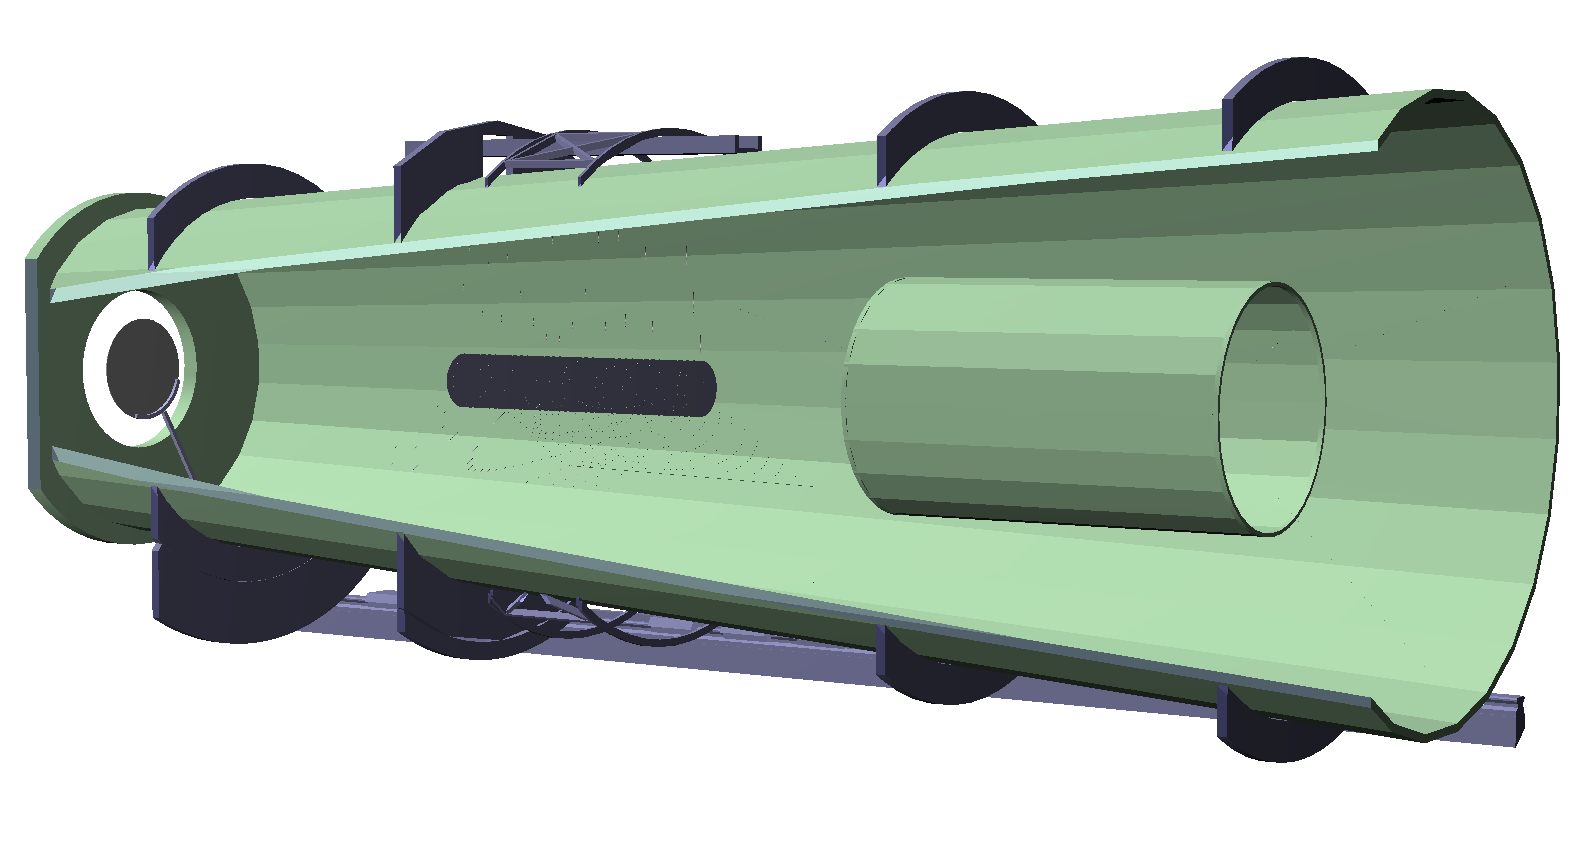
\includegraphics[width=0.95\textwidth]{png/ds2_cutout}
      }
    };
    % \node [text width=8cm, scale=1.0] at (14.5,0.5) {$\mu_B$, expected background mean};
    % \node [text width=8cm, scale=1.0, rotate={90}] at (1.5,7.5) { $S_{D}$, ``discovery'' signal strength  };
  \end{tikzpicture}
  \caption{
    \label{figure:ds2_cutout}
    TSdA is the disk on the left , next to the pion degrader
  }
\end{figure}

Neutrons are responsible for about 40\% of the total number of hits in the tracker.
For 1-batch booster mode, the total number of straw hits per event is expected to be
about 1,000, with about 400 hits resulting from neutrons.
In this mode, the total number of neutrons emitted per microbunch is about 30,000.
Given the TSdA dimensions, only about 1.5\% or about 450 neutrons would go through it.
Increasing the total number of hits in the tracker by 30\% would require
significant fraction of those neutrons to interact in the TS via a mechanism resulting 
in the secondary particles producing hits in the tracker.

To understand the mechanism of the underlying interaction, we attempted
to reproduce the results of \cite{MU2E_3479_NEUTRON_SHIELDING}.


%%%%%%%%%%%%%%%%%%%%%%%%%%%%%%%%%%%%%%%%%%%%%%%%%%%%%%%%%%%%%%%%%%%%%%%%%%%%%%
\section {Datasets}

We used branch=pbar2m of the Mu2e offline software, qualifier=p057.
For each of two geometries, with and without the TSdA, 3M single neutron events
have been generated, and simulated in the detector to produce the detector steps.
In the tracker, one detector step (so-called ``straw gas step'') in most cases
corresponds to one straw hit. In general, it is not true for the calorimeter, where
energy depositions of several particles in the same crystal could,
after the digitization, be combined into a single ``calorimeter hit'' much more often.
To simplify the analysis and keeping focus on the tracker, a detector step was considered
a proxy to a hit.

The datasets used in the analysis are described in Table~\ref{table:datasets}.
More details could be found in in Appendix~\ref{appendix_b}

\begin{table}[H]
  \centering {
\begin{tabularx}{0.6\textwidth} {|X|c|c|c|c|c|}  % 
% \begin{tabular}{1.0\textwidth} {|l|l|}  %
  \hline
  Dataset             & geometry  & $N_0$    & $N_1$  & f = $N_1/N_0$       \\
                      &           &          &        &                 \\
  \hline                                                                                          
  pipenu.neut0b0      &  default  &   3M     & 41940  &   $1.40e^{-2}$   \\
  \hline                                                                                          
  pipenu.neut1b0      &  no TSdA  &   3M     & 42581  &   $1.42e^{-2}$  \\
  \hline
  su2020.neut0        &  default  &  100,000 &  1462  &   $1.46e^{-2}$  \\
  \hline
\end{tabularx}
}
  \caption{
    \label{table:datasets}
    $N_0$ : the total number of generated events; 
    $N_1$: number of simulated events with at least one detector step 
  }
\end{table}

Table~\ref{table:datasets} shows that the number of single neutron events resulting
in hits in the detector doesn't really depend on the presence of TSdA - removing TSdA 
changes that number by 1.5\%.

The fraction of neutron events with hits, $f_H$, is about 1.4\%, and 
is within 5\% from the value used for the SU2020 simulation\cite{SU2020_DOC_MIXING}.

This suggests that TSdA doesn't stop a significant number of neutrons,
but rather plays a different role.


%%%%%%%%%%%%%%%%%%%%%%%%%%%%%%%%%%%%%%%%%%%%%%%%%%%%%%%%%%%%%%%%%%%%%%%%%%%%%%
\section{Neutron-induced occupancy in the tracker}

Figure~\ref{figure:figure_00021} shows distributions of different
parameters of the detector steps in the tracker - straw gas steps - with and without the TSdA.

The total numbers of steps are different by 4.4\%. With one straw gas step resulting
in one straw hit, the same statement should hold for the ratio of the number of straw hits.
%
As about 40\% of all hits have their origin traced back to neutrons, a 4.4\% increase of the
neutron contribution corresponds to 1.8\% increase of the total number of hits.
Both numbers are significantly lower than 30\% reported in \cite{MU2E_3479_NEUTRON_SHIELDING}.

A scan of few events contributing additional hits in a geometry w/o the TSdA showed that
the ``extra'' hits are due to low energy electrons resulting from a neutron capture in the TS,
which drifted into the tracker. With the TSdA present, the electrons stop in it.

\begin{figure}[H]
  \begin{tikzpicture}
    \node[anchor=south west,inner sep=0] at (0,0.) {
      % \node[shift={(0 cm,0.cm)},inner sep=0,rotate={90}] at (0,0) {}
      % \makebox[\textwidth][c] {
        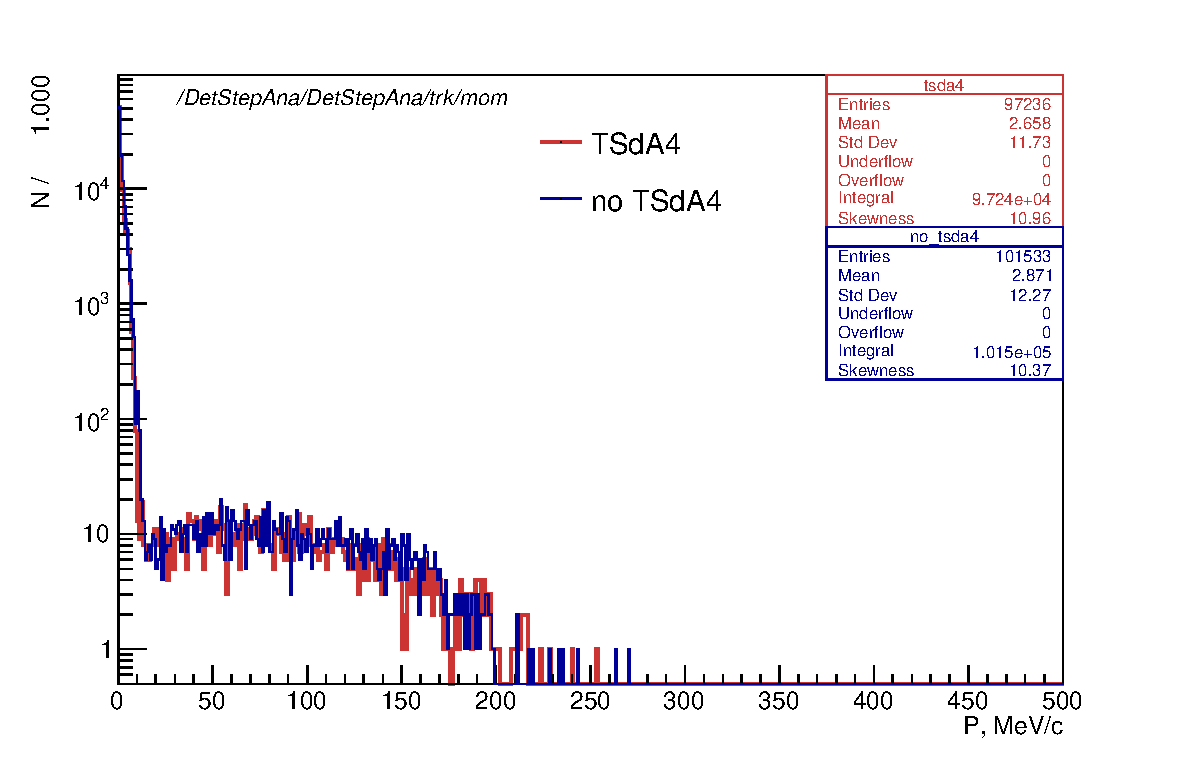
\includegraphics[width=0.55\textwidth]{pdf/figure_00021}
      % }
    };
    \node[anchor=south west,inner sep=0] at (10,0.) {
      % \node[shift={(0 cm,0.cm)},inner sep=0,rotate={90}] at (0,0) {}
      % \makebox[\textwidth][c] {
        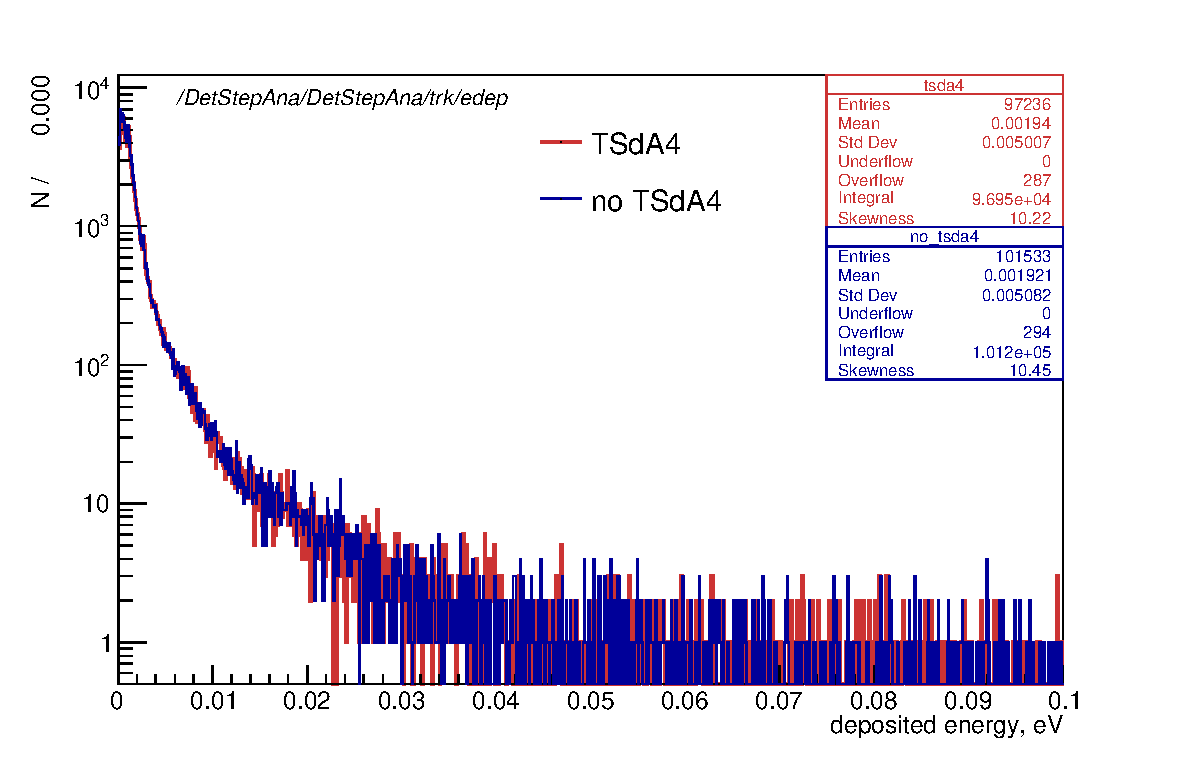
\includegraphics[width=0.55\textwidth]{pdf/figure_00022}
      % }
    };
    \node[anchor=south west,inner sep=0] at (0,-8.) {
      % \node[shift={(0 cm,0.cm)},inner sep=0,rotate={90}] at (0,0) {}
      % \makebox[\textwidth][c] {
        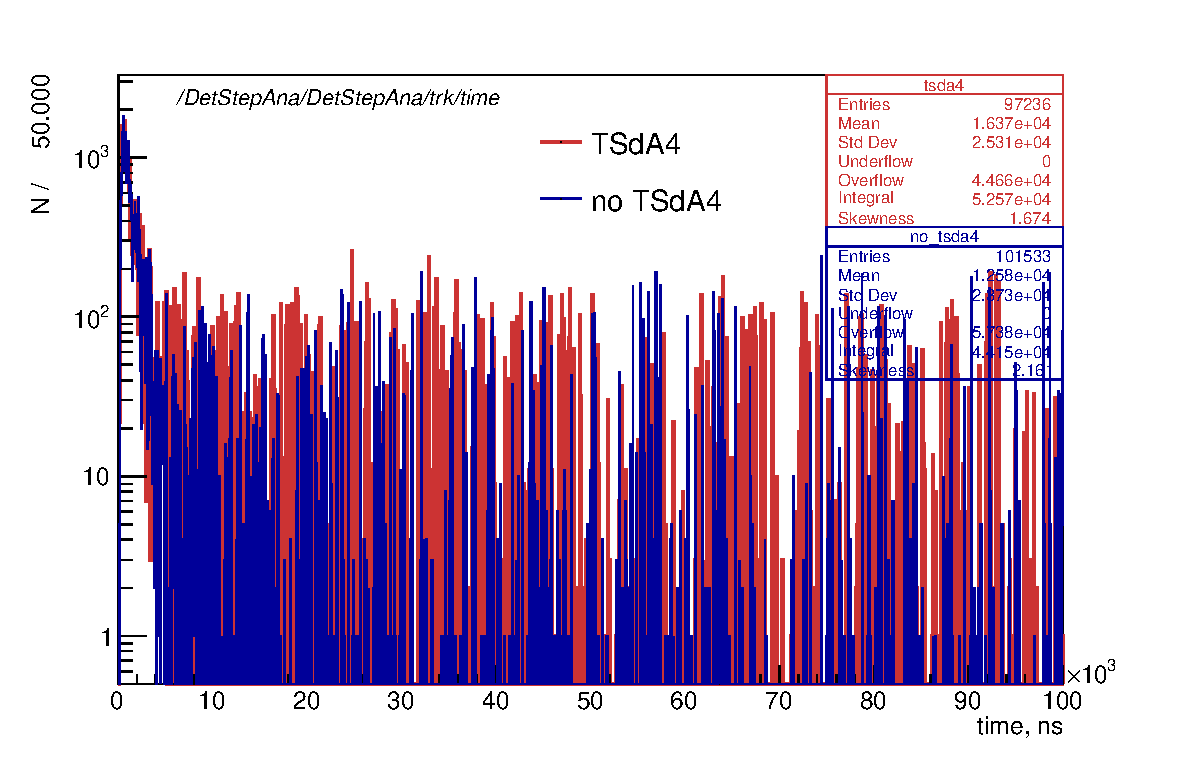
\includegraphics[width=0.55\textwidth]{pdf/figure_00023}
      % }
    };
    % \node [text width=8cm, scale=1.0] at (14.5,0.5) {$\mu_B$, expected background mean};
    % \node [text width=8cm, scale=1.0, rotate={90}] at (1.5,7.5) { $S_{D}$, ``discovery'' signal strength  };
  \end{tikzpicture}
  \caption{
    \label{figure:figure_00021}
    Distribution of \\
    a) momentum of the ``mother'' particle producing the hit.
    The distribution is dominated by low energy electrons \\
    b) per-step energy depositions in the tracker \\
    c) hit time distribution of straw gas steps due to neutron interactions
  }
\end{figure}

% \begin{figure}[H]
%   \begin{tikzpicture}
%     \node[anchor=south west,inner sep=0] at (0,0.) {
%       % \node[shift={(0 cm,0.cm)},inner sep=0,rotate={90}] at (0,0) {}
%       \makebox[\textwidth][c] {
%         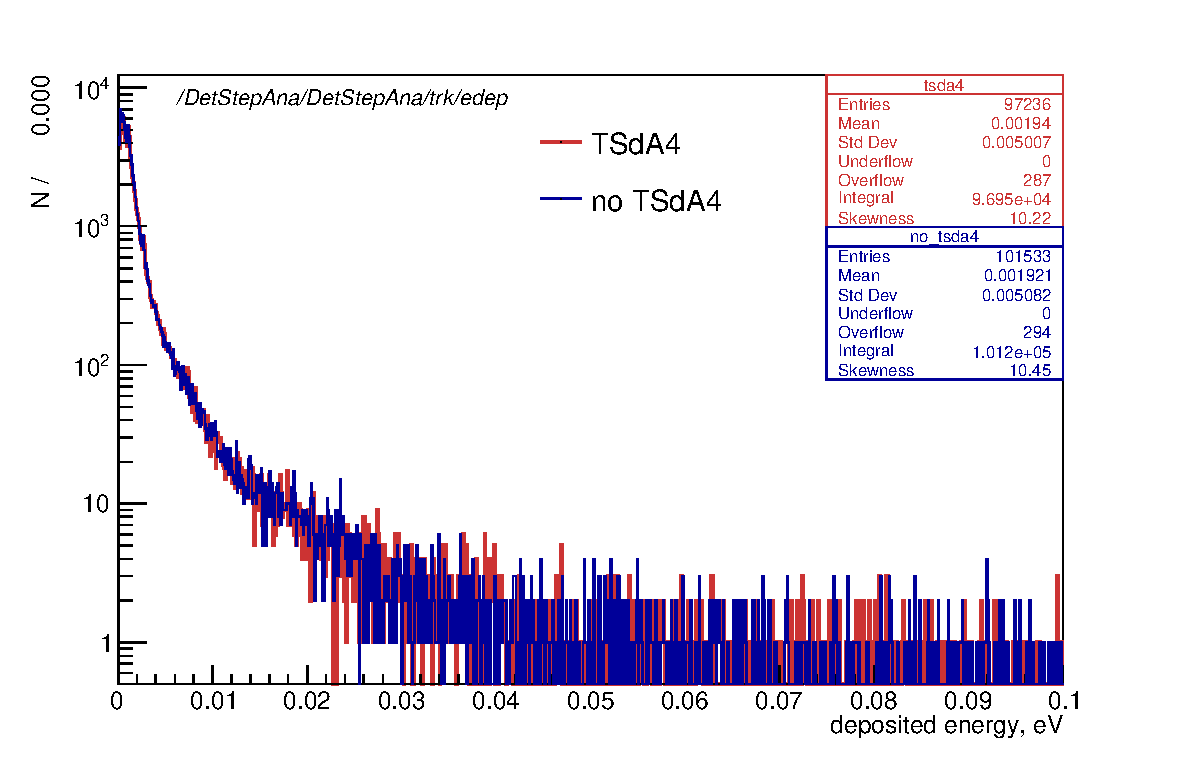
\includegraphics[width=0.95\textwidth]{pdf/figure_00022}
%       }
%     };
%     % \node [text width=8cm, scale=1.0] at (14.5,0.5) {$\mu_B$, expected background mean};
%     % \node [text width=8cm, scale=1.0, rotate={90}] at (1.5,7.5) { $S_{D}$, ``discovery'' signal strength  };
%   \end{tikzpicture}
%   \caption{
%     \label{figure:figure_00022}
%     Distribution of per-step energy depositions in the tracker
%   }
% \end{figure}

% \begin{figure}[H]
%   \begin{tikzpicture}
%     \node[anchor=south west,inner sep=0] at (0,0.) {
%       % \node[shift={(0 cm,0.cm)},inner sep=0,rotate={90}] at (0,0) {}
%       \makebox[\textwidth][c] {
%         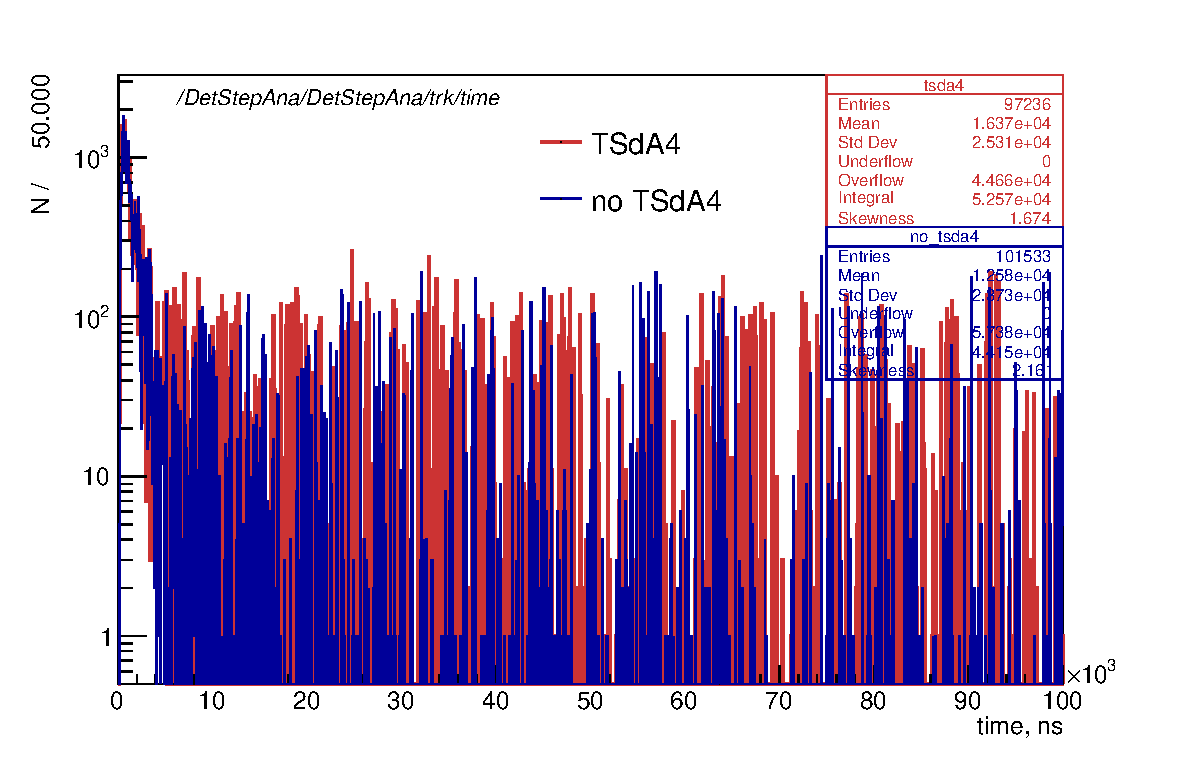
\includegraphics[width=0.95\textwidth]{pdf/figure_00023}
%       }
%     };
%     % \node [text width=8cm, scale=1.0] at (14.5,0.5) {$\mu_B$, expected background mean};
%     % \node [text width=8cm, scale=1.0, rotate={90}] at (1.5,7.5) { $S_{D}$, ``discovery'' signal strength  };
%   \end{tikzpicture}
%   \caption{
%     \label{figure:figure_00023}
%     hit time distribution of straw gas steps due to neutron interactions
%   }
% \end{figure}

%%%%%%%%%%%%%%%%%%%%%%%%%%%%%%%%%%%%%%%%%%%%%%%%%%%%%%%%%%%%%%%%%%%%%%%%%%%%%%
\newpage
\section{Neutron-induced occupancy in the calorimeter}

Figure~\ref{figure:figure_00031} shows distributions of different
parameters of the detector steps in the calorimeter for two geometries - with and without
the TSdA.
%
For both geometries, all distributions look very similar, and the relative difference
of 0.6\% between the total numbers of hits is negligible.

\begin{figure}[H]
  \begin{tikzpicture}
    \node[anchor=south west,inner sep=0] at (0,0.) {
      % \node[shift={(0 cm,0.cm)},inner sep=0,rotate={90}] at (0,0) {}
      % \makebox[\textwidth][c] {
        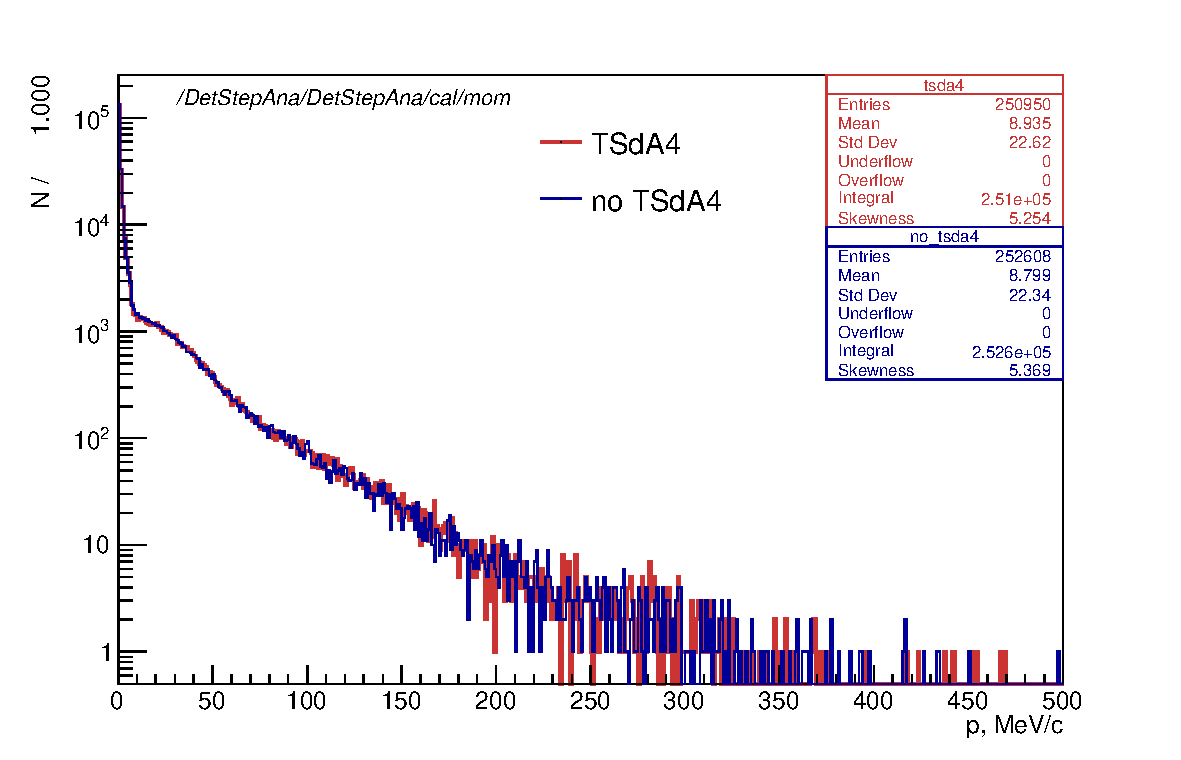
\includegraphics[width=0.55\textwidth]{pdf/figure_00031}
      % }
    };
    \node[anchor=south west,inner sep=0] at (10,0.) {
      % \node[shift={(0 cm,0.cm)},inner sep=0,rotate={90}] at (0,0) {}
      % \makebox[\textwidth][c] {
        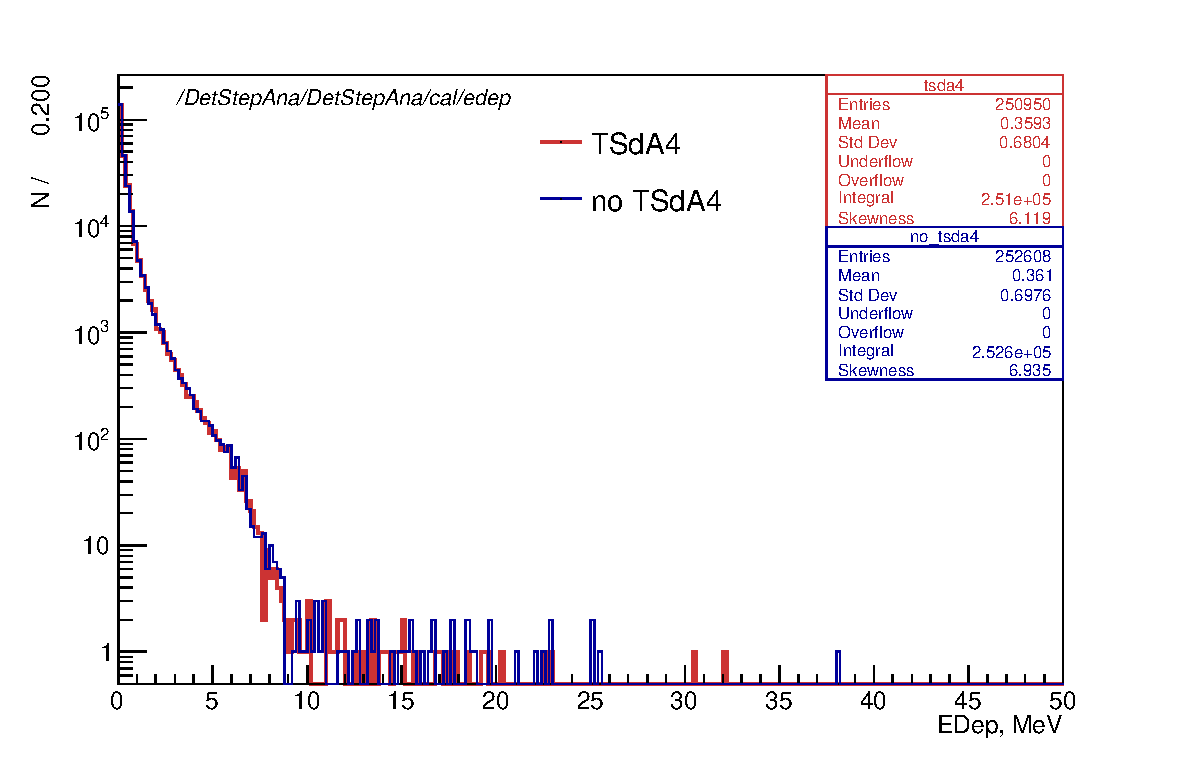
\includegraphics[width=0.55\textwidth]{pdf/figure_00032}
      % }
    };
    \node[anchor=south west,inner sep=0] at (0,-7.) {
      % \node[shift={(0 cm,0.cm)},inner sep=0,rotate={90}] at (0,0) {}
      % \makebox[\textwidth][c] {
        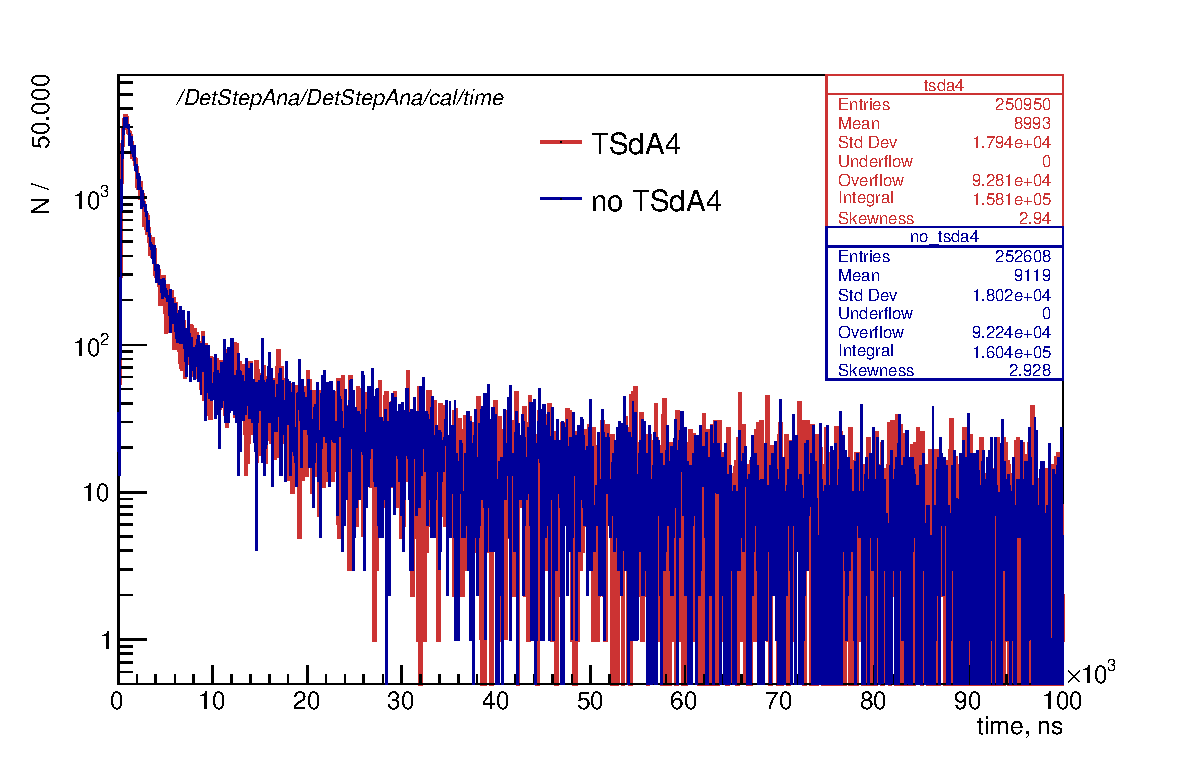
\includegraphics[width=0.55\textwidth]{pdf/figure_00033}
      % }
    };
    % \node [text width=8cm, scale=1.0] at (14.5,0.5) {$\mu_B$, expected background mean};
    % \node [text width=8cm, scale=1.0, rotate={90}] at (1.5,7.5) { $S_{D}$, ``discovery'' signal strength  };
  \end{tikzpicture}
  \caption{
    \label{figure:figure_00031}
    Distributions of \\
    a) momentum of the ``mother'' particle producing hits in the calorimeter.
    The distribution is dominated by neutrons from muon captures \\
    b) per-step energy depositions \\
    c) hit time 
  }
\end{figure}

% \begin{figure}[H]
%   \begin{tikzpicture}
%     \node[anchor=south west,inner sep=0] at (0,0.) {
%       % \node[shift={(0 cm,0.cm)},inner sep=0,rotate={90}] at (0,0) {}
%       \makebox[\textwidth][c] {
%         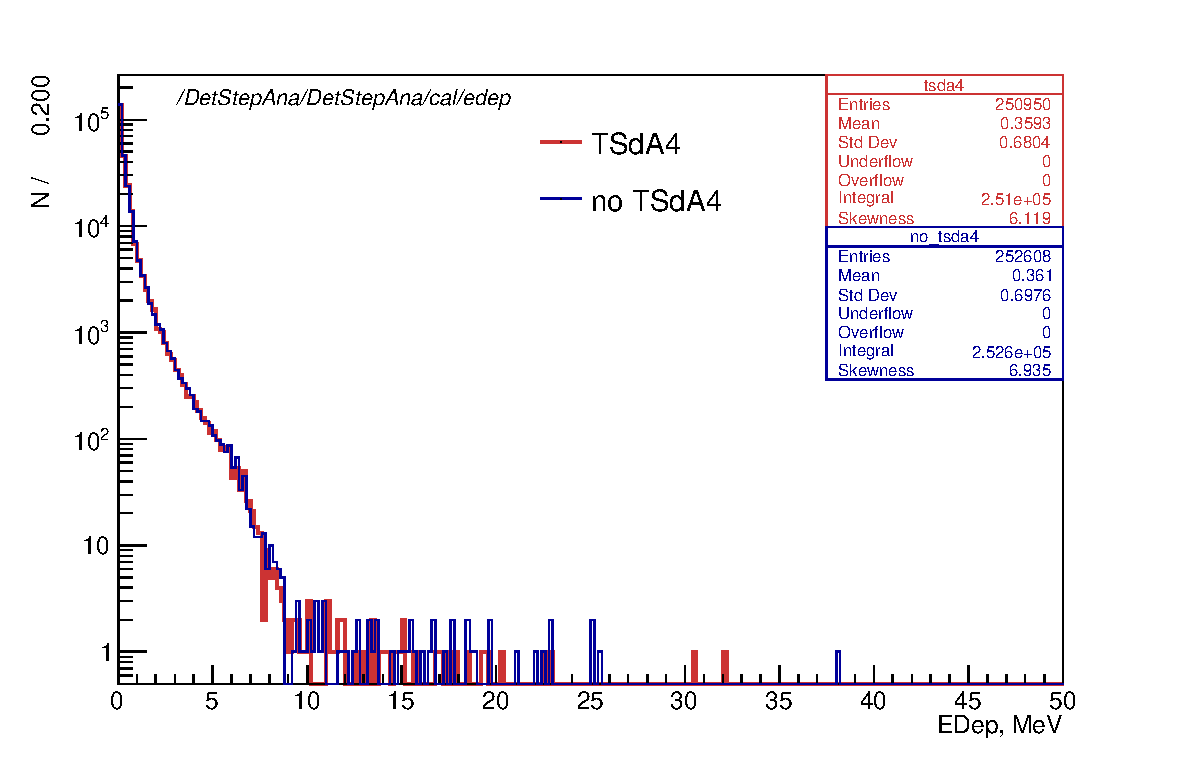
\includegraphics[width=0.95\textwidth]{pdf/figure_00032}
%       }
%     };
%     % \node [text width=8cm, scale=1.0] at (14.5,0.5) {$\mu_B$, expected background mean};
%     % \node [text width=8cm, scale=1.0, rotate={90}] at (1.5,7.5) { $S_{D}$, ``discovery'' signal strength  };
%   \end{tikzpicture}
%   \caption{
%     \label{figure:figure_00032}
%     Distribution of per-step energy depositions in the tracker
%   }
% \end{figure}

% \begin{figure}[H]
%   \begin{tikzpicture}
%     \node[anchor=south west,inner sep=0] at (0,0.) {
%       % \node[shift={(0 cm,0.cm)},inner sep=0,rotate={90}] at (0,0) {}
%       \makebox[\textwidth][c] {
%         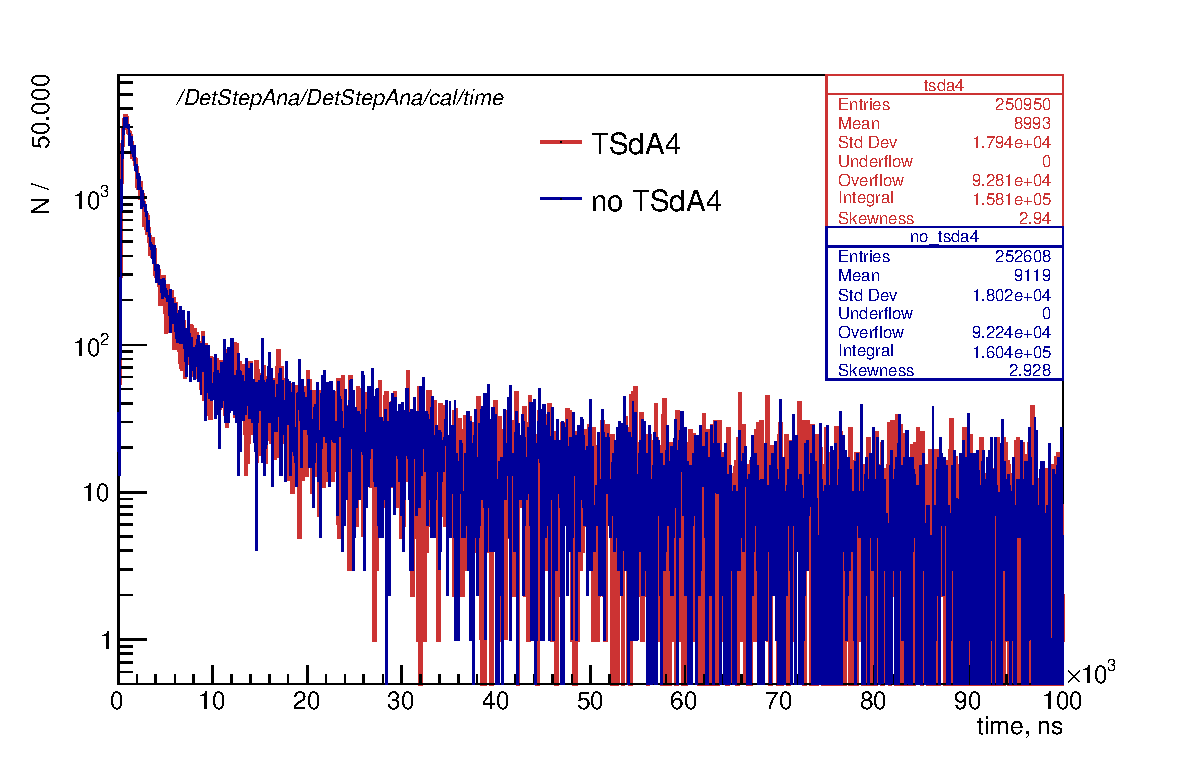
\includegraphics[width=0.95\textwidth]{pdf/figure_00033}
%       }
%     };
%     % \node [text width=8cm, scale=1.0] at (14.5,0.5) {$\mu_B$, expected background mean};
%     % \node [text width=8cm, scale=1.0, rotate={90}] at (1.5,7.5) { $S_{D}$, ``discovery'' signal strength  };
%   \end{tikzpicture}
%   \caption{
%     \label{figure:figure_00033}
%     hit time distribution of straw gas steps due to neutron interactions
%   }
% \end{figure}

%%%%%%%%%%%%%%%%%%%%%%%%%%%%%%%%%%%%%%%%%%%%%%%%%%%%%%%%%%%%%%%%%%%%%%%%%%%%%% 
\section {Summary}

We find that the TSd absorber has a minimal impact on the tracker hit load.
The scale of the impact is well within the physics uncertainties of the simulation:
\begin{itemize}
\item 
  w/o the TSdA, the tracker occupancy due to neutrons goes up
  by about 4\%.  That corresponds to less than 2\% change in the total number
  of hits in the tracker.
\item 
%
  The impact of the TSdA on the calorimeter occupancy is negligible,
  less than 1\%.
\end{itemize}

%%%%%%%%%%%%%%%%%%%%%%%%%%%%%%%%%%%%%%%%%%%%%%%%%%%%%%%%%%%%%%%%%%%%%%%%%%%%%%
%
%%%%%%%%%%%%%%%%%%%%%%%%%%%%%%%%%%%%%%%%%%%%%%%%%%%%%%%%%%%%%%%%%%%%%%%%%%%%%%
\newpage
\bibliographystyle{unsrtnat}
\bibliography{clfv,mu2e_internal_notes,mu2e_piplusenu_notes,su2020_notes,radiative_pion_capture}

% \include{appendix_a}
\appendix

%%%%%%%%%%%%%%%%%%%%%%%%%%%%%%%%%%%%%%%%%%%%%%%%%%%%%%%%%%%%%%%%%%%%%%%%%%%%%%
\section {Datasets}
\label{appendix_b}
\begin{itemize}
\item 
  Definition of the datasets used for this study ant the book-keeping information
  can be found at \\
  \href{https://github.com/sridhar130/pipenu}{https://github.com/sridhar130/pipenu}.
\item
  the datasets and stntuples are available from {\bf /exp/mu2e/data/projects/pipenu}
\item
  location of the stntuple catalogs : \\
  \href{https://mu2e.fnal.gov/public/hep/computing/Stntuple/cafdfc/pipenu/index.shtml}
  {https://mu2e.fnal.gov/public/hep/computing/Stntuple/cafdfc/pipenu/index.shtml}
\end{itemize}

%%% Local Variables:
%%% mode: latex
%%% TeX-master: "mu2e-xxxxx"
%%% End:


\end{document}
